\documentclass[UTF8, a4paper, 11pt]{article}
\usepackage{diagbox}
\usepackage{subcaption}
\usepackage[UTF8, scheme=plain]{ctex}
\usepackage{fontspec}
\usepackage{float}
\usepackage{amsmath}
\newtheorem{myDef}{Definition}
\usepackage{graphicx}
\usepackage{geometry}
\usepackage{listings}
\usepackage{xcolor}
\usepackage{caption}
\geometry{scale=0.8}
\linespread{1.5}
\usepackage{hyperref}
\usepackage{color}
\usepackage{fontspec}
\usepackage{enumitem}
\usepackage[linesnumbered,boxed]{algorithm2e}    
\usepackage{xeCJK}
\usepackage{indentfirst} 
\graphicspath{{Pics/}} 	% 在于.tex同级的目录下创建名为pic的文件夹,存放图片


\setlength{\parindent}{2em}

\lstset{
    language={python},
    frame=shadowbox,
    breaklines=true,
    numbers=left,
    backgroundcolor=\color[RGB]{245,245,244},
    rulesepcolor=\color{red!20!green!20!blue!20},
    numberstyle={\color[RGB]{0,192,192}\tiny},
    basicstyle=\footnotesize \fontspec{Source Code Pro}
}
\setenumerate[1]{itemsep=0pt,partopsep=0pt,parsep=\parskip,topsep=0pt}
\setitemize[1]{itemsep=0pt,partopsep=0pt,parsep=\parskip,topsep=0pt}
\setdescription{itemsep=0pt,partopsep=0pt,parsep=\parskip,topsep=0pt}


\title{	
\normalfont \normalsize
\textsc{School of Data and Computer Science, Sun Yat-sen University} \\ [25pt] %textsc small capital letters
\rule{\textwidth}{0.5pt} \\[0.4cm] % Thin top horizontal rule
\huge 作业2\\ % The assignment title
\rule{\textwidth}{2pt} \\[0.5cm] % Thick bottom horizontal rule
\author{18308045 谷正阳}
\date{\normalsize\today}
}

\begin{document}
\maketitle
\tableofcontents
\newpage
\section{CUDA实现}
\subsection{程序整体逻辑}
每个线程处理一个点周围$5\times5$邻域内有效数字(指在输入矩阵边界内的)的熵。

要计算熵,线程内部需先串行地统计$5\times5$邻域内总有效数字个数,各个有效数字的个数。
假设$num$为总有效数字个数,$5\times5$邻域在与输入矩阵边界不相交的情况下,$num=5\times5=25$。
当与输入矩阵边界相交的情况下,在边界内的邻域部分也是一个矩形。
假设当前点为$(tx,ty)$,该点邻域与左边相交,则矩形宽度为$5\times(tx+3)$。
类似地,可以得出大小为$m\times n$输入矩阵内任意点$(tx,ty)$的邻域与该输入矩阵相交的矩形大小:
\begin{equation}
    num=(\min(ty,2)+\min(m-ty2,3))\times(\min(tx,2)+\min(n-tx2,3)).
\end{equation}
此即总有效数字的个数。各个有效数字的个数则通过统计图$h$表示,对于数字$i$,其出现次数为$h[i]$。

结合上述统计,熵计算公式可做如下变换:
\begin{equation}
    \begin{aligned}
    H(X_{tx,ty})=&\sum_{i=0}^{15}
    \begin{cases}
        0,&\text{if }h[i]=0\\
        -\frac{h[i]}{num}\cdot\log(\frac{h[i]}{num}),&\text{otherwise}
    \end{cases}\\
    =&\frac{
        \sum_{i=0}^{15}
        \begin{cases}
            0,&\text{if }h[i]=0\\
            -h[i]\cdot\log(h[i]),&\text{otherwise}
        \end{cases}
    }{-num}+\log(num)
    \end{aligned}.
    \label{eq:HX}
\end{equation}
\subsection{设计存储器类型}
程序涉及了全局内存,本地内存,寄存器,只读/纹理内存,共享内存。
本地内存、寄存器在此不做讨论。
\subsubsection{全局内存}
全局内存用于存储输入矩阵和输出矩阵。
其特点是访问慢,默认会通过二级缓存读写。
同一线程束中二级缓存读写以内存事务进行,数据最好对齐,且步长不宜过大。
在这里数据是int或float类型,都是4Bytes是对齐的因此不做讨论。
而对步长而言,对x方向相邻(在全局内存上相邻,步长为1)的全局内存并行访问。
\subsubsection{只读/纹理内存}
只读/纹理内存,在开普勒架构以后使用线程块独立的只读缓存对其读写,在数据量比较小的情况下可以很好地利用缓存资源。
我电脑的显卡如下
\begin{figure}[H]
    \centering
    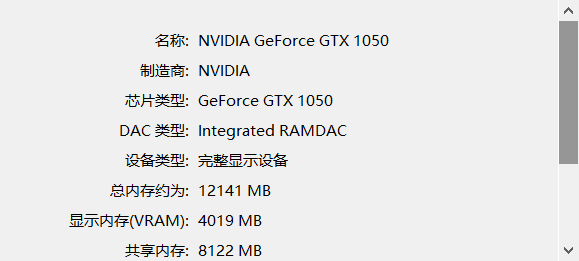
\includegraphics[width=0.9\textwidth]{显卡1.png}
\end{figure}
,是开普勒架构以后的帕斯卡架构,使用只读/纹理内存利于提高效率。
另外纹理内存可以关注到高维的空间局部性,契合此问题中对邻域块的访问的高维的空间局部性,因而用来作为改进点。
\subsubsection{共享内存}
实际上是线程块独立的可编程缓存,线程块内线程可以对其高速读写。
同一线程束对其访问可能出现存储体冲突的问题。
假设步长为$stride$,$i$遍历$[0,31]$($32$的剩余系),要满足$i\cdot stride$两两不同余才能保证不发生存储体冲突。
这等价于$32$和$stride$的最大公因数是$1$,因而需要$stride$是奇数。

每个线程块在计算熵之前可以将输入矩阵中用到的部分从全局内存读入共享内存,这样线程块内线程可以高速地读取用到的输入矩阵的值。
假设线程块大小为$BDIM\_Y\times BDIM\_X$,用到的数据需要向外扩展2层即$(BDIM\_Y+2)\times(BDIM\_X+2)$。
此处线程束内对其访问步长为$1$,因而不会发生存储体冲突。
\subsection{查表对数运算}
根据公式\ref{eq:HX},进行对数运算的数都是$[1,25]$的整数,因而查表是可行的。
另外在此可以定义表第$0$项为$0$,假设表为$logt$,这样公式\ref{eq:HX}可简化为:
\begin{equation}
    H(X_{tx,ty})=\frac{\sum_{i=0}^{15}-h[i]\cdot logt[h[i]]}{-num}+logt[num].
\end{equation}
对性能的影响会在后面讨论。
\subsection{实验}
设定输入矩阵大小$2048\times2048$,使用不同版本的核函数做运算,每个矩阵计算$100$次算平均时间,并用check\_result检查并输出结果正确性。
\begin{figure}[H]
\begin{center}
\begin{subfigure}[b]{0.48\linewidth}
    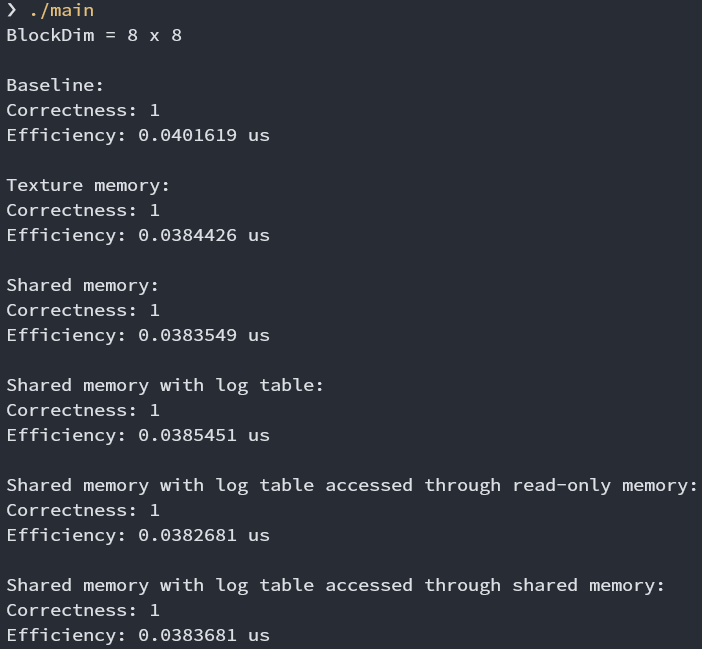
\includegraphics[width=\textwidth]{8.png}
\end{subfigure}
\begin{subfigure}[b]{0.48\linewidth}
    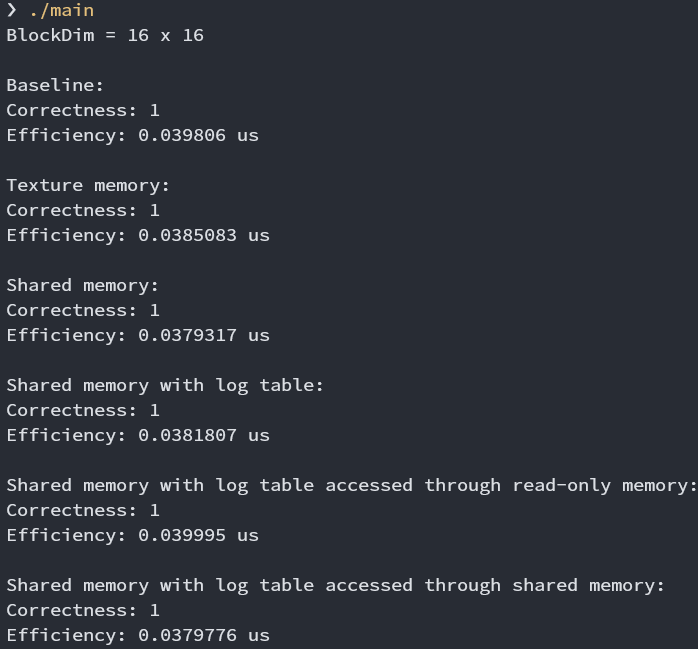
\includegraphics[width=\textwidth]{16.png}
\end{subfigure}
\begin{subfigure}[b]{0.48\linewidth}
    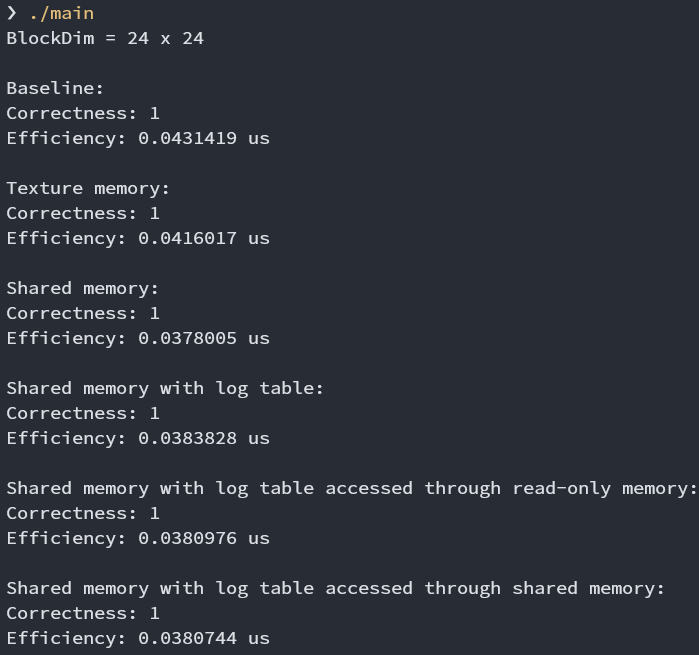
\includegraphics[width=\textwidth]{24.png}
\end{subfigure}
\begin{subfigure}[b]{0.48\linewidth}
    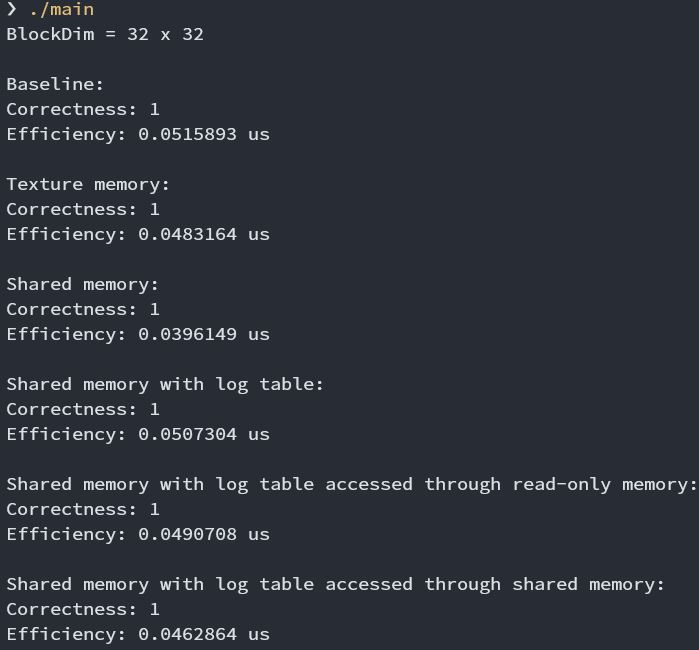
\includegraphics[width=\textwidth]{32.png}
\end{subfigure}
\end{center}
\end{figure}
发现总的来说,共享内存快于纹理内存快于全局内存,而且块小时纹理内存速度接近共享内存,块大时纹理内存速度接近全局内存。
原因是共享内存是可编程的缓存,在这里没有定义替换操作因而只需读一次全局内存。
纹理内存除二级缓存还会使用线程块独立的只读缓存,在块小时线程块需要读取的数据量小,无需过多替换,在块大时需要读取的数据量大,仍需要一些替换操作。
全局内存使用二级缓存,不同线程块共用需要更多的替换操作即需要更多访问全局内存。
另外,在块的左边和上边的线程还需负责拷贝共享内存最外两层(即线程块外两层)的数据,这里并行程度比拷贝中间区域低,因而运行慢。
在块小的时候,边上线程占的比例比较大,因而共享内存拷贝费时,加速效果不明显,而块大时边上线程占比小,导致共享内存加速效果明显。

对$logt$的访问也符合这个规律,即共享内存快于只读内存快于全局内存。
但查$logt$方法求对数速度慢于调用$logf$直接计算,可能原因是$logf$计算所用到的指令时钟延迟短于访存操作。
\subsection{总结}
这次实验得到的经验如下:
\begin{enumerate}
\item 共享内存效率很高。
\item 在数据量小时可以使用纹理内存,效率接近共享内存且编程方便。
\item 一些运算(如对数)比访存更快。
\end{enumerate}
影响CUDA的因素如下
\begin{enumerate}
\item 活跃线程块数,如果每个线程块占用资源太多,如线程块过大,会导致运行变慢。
\item 存储的选择,减少访存数,尽量多的使用片上存储。
\item 分支的多少,共享内存拷贝外两层那里实际使用了分支,分支导致线程束上并行程度低,另外由于下面还有个线程块同步指令,所以实际上也影响了线程块级别上的并行程度。
\item 运算的多少,这里展开循环减少了计数器等不必要的运算,增加了效率。
\item 任务的划分要合理,每个线程的工作要适度,以掩盖延迟。
\end{enumerate}
\section{OpenMp实现}
本身check\_result用CPU实现,在这里只需把它用parallel for并行即可。
Number of loops表示被作用parallel for的循环迭代次数,Number of threads表示线程数。
\begin{figure}[H]
\begin{center}
\begin{subfigure}[b]{0.48\linewidth}
    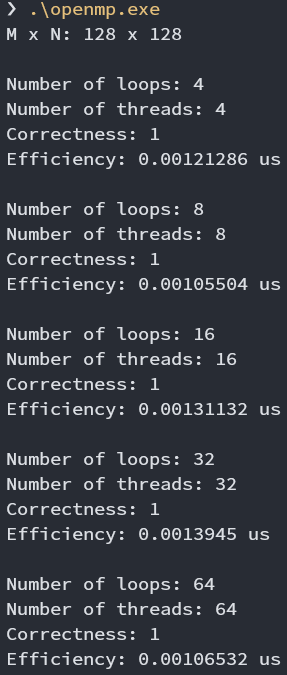
\includegraphics[width=\textwidth]{omp128.png}
\end{subfigure}
\begin{subfigure}[b]{0.48\linewidth}
    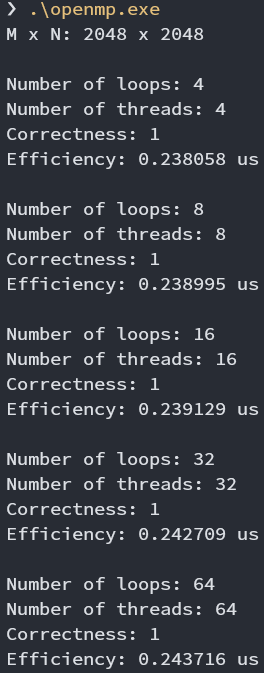
\includegraphics[width=\textwidth]{omp2048.png}
\end{subfigure}
\end{center}
\end{figure}
\begin{figure}[H]
\begin{center}
\begin{subfigure}[b]{0.48\linewidth}
    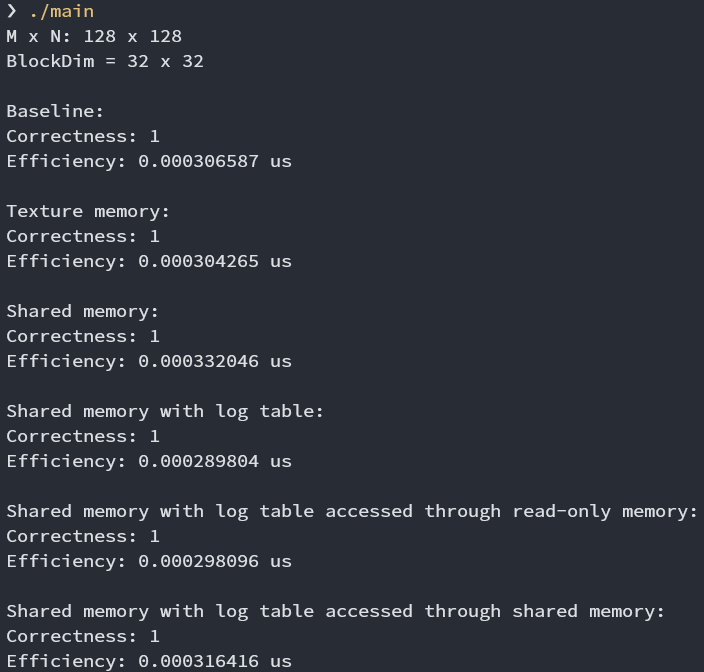
\includegraphics[width=\textwidth]{cuda128.png}
\end{subfigure}
\begin{subfigure}[b]{0.48\linewidth}
    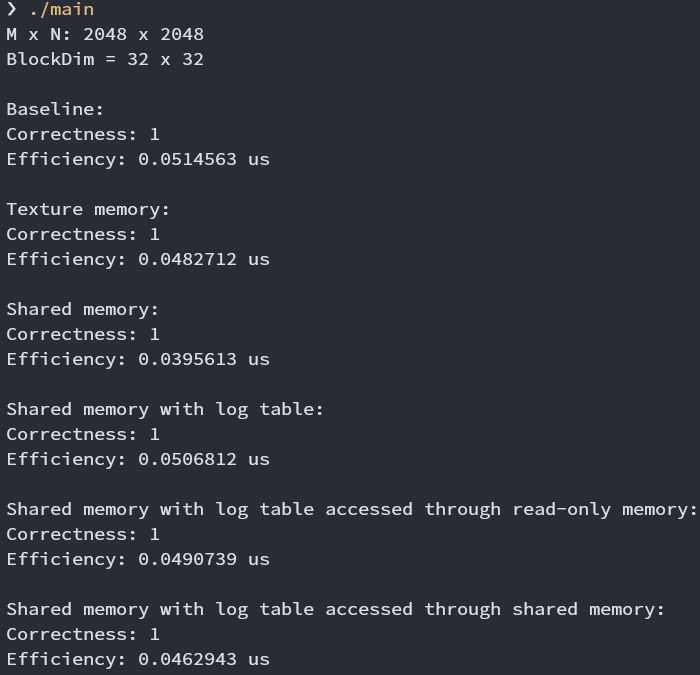
\includegraphics[width=\textwidth]{cuda2048.png}
\end{subfigure}
\end{center}
\end{figure}
不论是在大矩阵$2048\times2048$还是小矩阵$128\times128$,OpenMp效率都不如CUDA。
猜测是存储问题,这个问题需要分块处理,是高维的空间局部性,而行上的空间局部性被破坏,而CPU的缓存每次成行读入,不相复合。
%\clearpage
%\bibliography{E:/Papers/LiuLab}
%\bibliographystyle{apalike}
\end{document}
%%% Local Variables:
%%% mode: latex
%%% TeX-master: t
%%% End:
